\documentclass{article}

% spelling
\usepackage[english]{babel}

% page layout
\usepackage[letterpaper,top=2cm,bottom=2cm,left=2cm,right=2cm,marginparwidth=1.75cm]{geometry}

% math
\usepackage{amsmath}
\usepackage{amssymb}

% layout
\setlength\parindent{0pt}
\newcommand{\forceindent}{\leavevmode{\parindent=1em\indent}}
\usepackage{parskip}
\usepackage{setspace}
\onehalfspacing
\usepackage{graphicx}

% referencing
\usepackage[colorlinks=true, allcolors=black]{hyperref}
\usepackage[capitalize, nameinlink]{cleveref}
\crefdefaultlabelformat{#2\textbf{#1}#3} % 
\crefname{figure}{\textbf{Figure}}{\textbf{Figures}}
\Crefname{table}{\textbf{Table}}{\textbf{Tables}}

% captions
\usepackage[labelfont=bf]{caption}
\usepackage[table]{xcolor}

% tables
\usepackage{booktabs}
\renewcommand{\arraystretch}{1.25} % vertical spacing


\begin{document}

\begin{titlepage}
        \vspace*{1cm}
            
        \LARGE
        \textbf{Transmission of \emph{Mycobacterium tuberculosis (\emph{Mtb})} in a primary care clinic in South Africa before and during the COVID-19 pandemic: Comparing molecular, clinical, environmental, and patient tracking data from two observational field studies}
            
        \vspace{0.5cm}
        \Large
        Statistical analysis plan (SAP)
            
        \vspace{1.5cm}
            
        \textbf{SAP authors:} Nicolas Banholzer$^{1*}$, Lukas Fenner$^1$ \\
        \textbf{Study authors:} Nicolas Banholzer$^{1*}$, Keren Middelkoop$^{2}$, Juane Leukes$^{2}$, Kathrin Z\"urcher$^{1}$, Robin Wood$^{2}$, Matthias Egger$^1$, Lukas Fenner$^1$

        \vspace{1cm}

        $^1$ Institute of Social and Preventive Medicine, University of Bern, Switzerland \\
        $^2$ Desmund Tutu HIV Centre, University of Cape Town, South Africa \\
        $^*$ Corresponding author: nicolas.banholzer@unibe.ch
            
        \vfill
            
        \Large
        Version number: 0.3 \\
        Version date: \today 

        \vspace*{1cm}
\end{titlepage}

\tableofcontents

\clearpage

\section{Introduction}

This document describes the proposed presentation and analysis for the main paper(s) reporting results from a study estimating and comparing the transmission of \emph{Mycobacterium tuberculosis (\emph{Mtb})} in a primary care clinic in Cape Town (South Africa) before and during the COVID-19 pandemic. Various infection control measures were introduced during the COVID-19 pandemic, including restricted patient flows, general mask-wearing, and improved ventilation. To assess the effects of these measures, the following data were collected during both study periods:

\begin{enumerate}
    \item \textbf{Molecular data}: Bioaerosol samples to detect respiratory infectious particles in the air, particularly \emph{Mtb} particles.
    \item \textbf{Clinical data}: Number of registered patients, presumptive TB cases, and diagnosed TB patients. 
    \item \textbf{Environmental data}: CO$_2$, relative humidity, and temperature.
    \item \textbf{Patient tracking}: Patient movements in the waiting and tuberculosis (TB) room of the clinic, to monitor person-time in the clinic.
\end{enumerate}
 
Any deviations from the statistical analysis plan will be described and justified in the final report. The analysis will be carried out by identified, appropriately qualified and experienced statisticians, who will ensure the integrity of the data during their processing. 

\section{Background}

In a previous study, we estimated the risk of \emph{Mtb} transmission in a primary care clinic in South Africa between July and August 2019\cite{Zurcher2022JID}. The study design, measurements, and setting were described in a protocol before the study commenced \cite{Zurcher2020BMJ}. We repeated the study in the same clinic between October and November 2021 (during the COVID-19 pandemic). Multiple infection control measures were put in place during this time:

\begin{itemize}
    \item \textbf{Restricted patient flows}: Patients received fixed appointments to avoid crowding and reduce waiting times at the clinic.  They were asked to arrive at the earliest one hour before the appointment, otherwise, they were asked to wait outside the clinic. In addition, clinical attendees with respiratory symptoms were tested outside the clinic before entering.
    \item \textbf{Mask-wearing}: Compulsory mask-wearing for all clinical attendees and staff members, except young children.
    \item \textbf{Active ventilation}: Opening of all windows and doors in the clinic throughout the day, to actively increase natural ventilation.
\end{itemize}


\subsection{Objectives of the study}

The primary objective of the study is to assess and compare the risk of \emph{Mtb} infection in the primary care clinic between the period before (2019) and during the COVID-19 pandemic (2021), and to assess the individual effects of the pandemic-related infection control measures. 

\subsection{Primary outcome}

The concentration of \emph{Mtb} genomes in bioaerosol samples expressed as DNA copies per microliter per hour of sampling.  


\subsection{Secondary outcomes}

\begin{enumerate}
    \item Proportion of diagnosed TB patients among registered patients.
    \item Proportion of presumptive TB patients among registered patients.
    \item Ventilation or outdoor air change rate (computed from indoor CO$_2$ levels and room occupancy).
    \item Person-time in the clinic. 
\end{enumerate}

\subsection{Variables}

\begin{enumerate}
    \item Molecular data (daily)
    \begin{enumerate}
        \item Number of \emph{Mtb} genomes in bioaerosol samples (DNA copies per microliters per hour of sampling)
        \item Number of other detected respiratory infectious particles in the air (copies per microliters), including SARS-CoV-2 and influenza. 
    \end{enumerate}
    \item Clinical data (daily)
    \begin{enumerate}
        \item Number of registered patients.
        \item Number of presumptive TB patients.
        \item Number of newly diagnosed TB patients.
    \end{enumerate}
    \item Environmental data (daily by minute)
    \begin{enumerate}
        \item CO$_2$ (parts per million [ppm]).
        \item Relative humidity (\%) and temperature (°C).
    \end{enumerate}
    \item Patient tracking data (daily by second)
    \begin{enumerate}
        \item Time and location of people in the clinic (observation ID, timestamp, x- and y-coordinates of the location).
    \end{enumerate}
    \item Building data
    \begin{enumerate}
        \item Width, breadth, height, and volume of the waiting and TB room of the clinic.
    \end{enumerate}
    \item Secondary data
    \begin{enumerate}
        \item Estimated incidence/prevalence of TB \cite{WHO2022TBReport}.
    \end{enumerate}
\end{enumerate}

\subsection{Hypothesis framework}

The null hypothesis will be that there is no true difference in the outcomes between the two studies. We will use a Bayesian framework to assess the null hypothesis and use the posterior distribution of the parameter modeling the difference in the outcome by study year to assess the direction and magnitude of the effects of the pandemic-related infection control measures that were implemented in the clinic. 

\subsection{Research hypotheses}

Our hypothesized links between pandemic-related infection control measures and the concentration of \emph{Mtb} in bioaerosol samples are illustrated with a direct acyclic graph (DAG) model (\Cref{fig:dag}). In the following, we develop our research hypotheses about the effects of infection control measures on the number of \emph{Mtb} DNA copies per microliter per hour of sampling time. 

First, the number of \emph{Mtb}-containing particles in the air depends on the generation of infectious particles. The total amount of particles generated depends on the person-time of infectious people in the clinic. Person-time in the clinic was aimed to be reduced by restricted patient flows. Therefore, this intervention should reduce the generated amount of infectious particles by clinical attendees. \medskip

\forceindent \textbf{Hypothesis 1}: Restricted patient flows decreased the number of \emph{Mtb} DNA copies per microliter per hour of sampling time. \medskip


Mask-wearing reduces the number of infectious particles exhaled into the air (and may also reduce the number of inhaled particles from the air). \medskip

\forceindent \textbf{Hypothesis 1}: Mask-wearing decreased the number of \emph{Mtb} DNA copies per microliter per hour of sampling time. \medskip

Second, the detection of \emph{Mtb} in bioaerosols depends on the survival of \emph{Mtb} over time, which depends on multiple environmental factors such as airflow, ventilation, humidity, and UV radiation \cite{Wang2021Science}. More active natural ventilation should accelerate the removal of infectious particles from the indoor air. \medskip

\forceindent \textbf{Hypothesis 1}: Active natural ventilation decreased the number of \emph{Mtb} DNA copies per microliter per hour of sampling time. \medskip

Ventilation may also affect other variables such as humidity, but the net effect on the generation and survival of infectious particles in the air is unclear \cite{Wang2021Science}. We, therefore, do not develop a hypothesis for the effect of ventilation via humidity on the number of \emph{Mtb} DNA copies per microliter per hour of sampling time. Nevertheless, we will adjust for a potential effect during analysis.

Our hypothesized effects are subject to potential unmeasured confounding and measurement error: 

\begin{itemize}
    \item The person-time of infectious people in the clinic is unknown. We estimate this latent variable during modeling, considering the number of diagnosed TB patients and by making assumptions on the unknown number of undiagnosed TB patients. 
    \item It is possible that \emph{Mtb} transmission was lower during the COVID-19 pandemic (e.g. due to social distancing measures). However, it seems more likely that TB was under-diagnosed during the COVID-19 pandemic due to fewer people visiting the clinic \cite{Soko2021EID,Pillay2021SAMJ,Uwishema2022DMPHP}. People afraid of getting infected may have postponed their regular clinical visits, resulting in a smaller total number of clinical visits during the COVID-19 pandemic. We, therefore, adjust the effect of restricted patient flows on the person-time in the clinic for the daily number of registered patients.
    \item The generation of infectious particles depends also on the individual infectiousness of infected people. More infectious individuals may generate more infectious particles per minute. The individual infectiousness of diagnosed TB patients is unknown.
	The removal of infectious particles depends not only on ventilation and humidity but also other, unmeasured environmental factors. For example, airflows may trap infectious particles in certain locations of the clinic \cite{Wang2021Science}. Spatial variation in the concentration of infectious particles may introduce small measurement errors due to the fixed location of the bioaerosol sampling devices in each room of the clinic, yet the placement of the bioaerosol sampling devices was the same in both study years.
    \item The two studies that we compared were conducted between slightly different time periods, i.e. July to late August (before the pandemic) vs October to early November (during the pandemic), which possibly introduces seasonal effects. However, the weather conditions were comparable (only 1-2 months difference) and the infection control measures were maintained during the pandemic independent of the season.
\end{itemize}

\begin{figure}[!htpb]
    \centering
    \caption{Directed acyclic graph (DAG) model showing the causal pathways from pandemic-related infection control measures (interventions) to the number of \emph{Mtb} DNA copies per microliter per hour of sampling time (measured outcome), which is a proxy for the risk of infection (unmeasured outcome) in the clinic.}
    \label{fig:dag}
    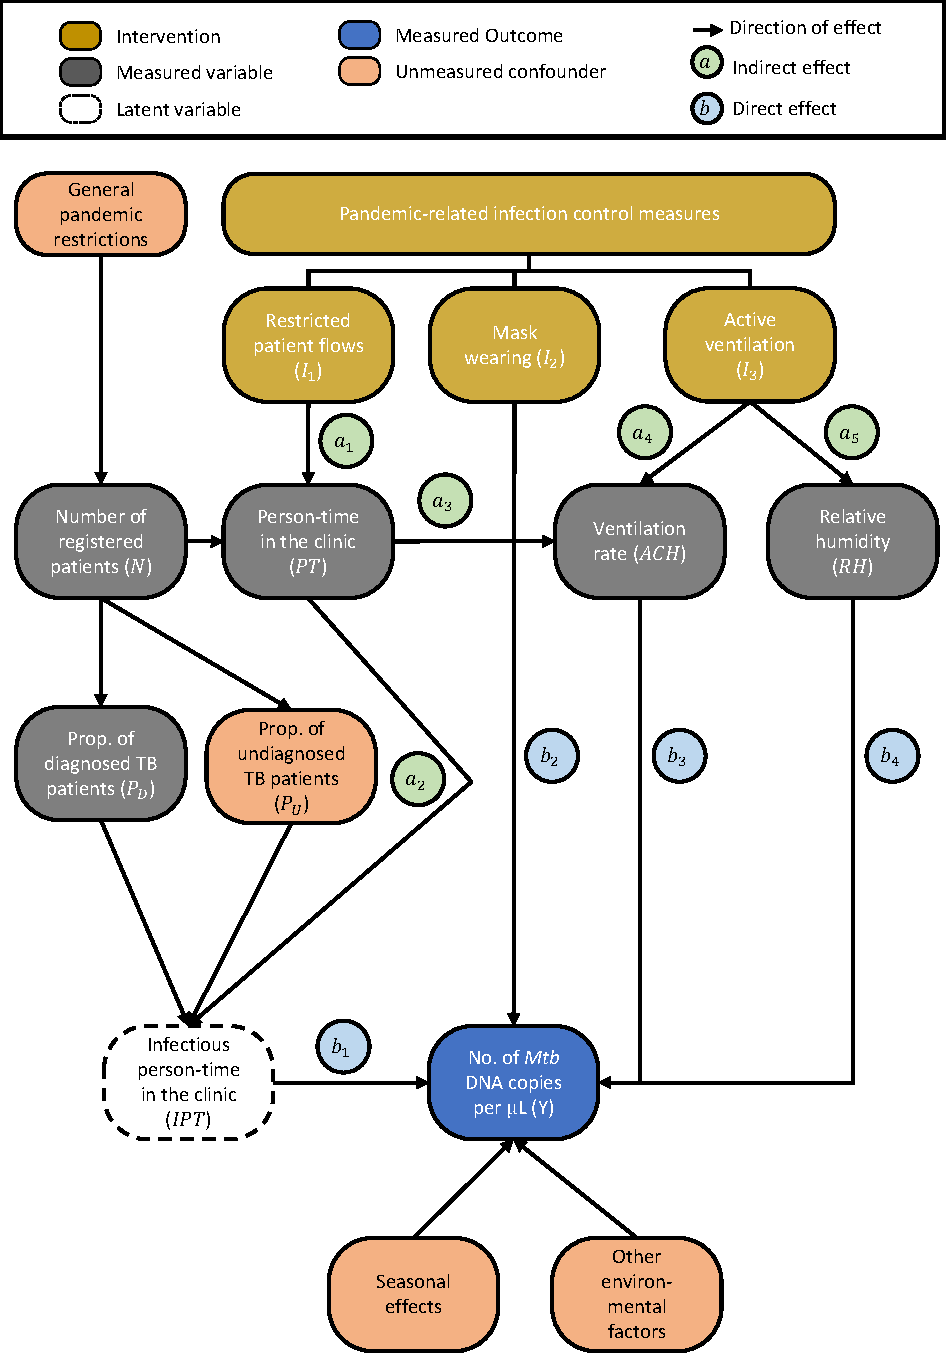
\includegraphics[width=.8\linewidth]{dag.pdf}
\end{figure}
	
\section{Study populations}

The target population includes all clinical attendees of the primary care clinic in South Africa between July and August 2019 (before the COVID-19 pandemic) and between October and November 2021. The primary outcome is the number of \emph{Mtb} DNA copies per microliter per hour of sampling time. The sampling time was 2h in 2019 and 3h in 2021. Samples were collected twice per day, unless the clinic was closed in the morning or afternoon, corresponding to 4h and 6h of sampling, respectively. By daytime, we have 39 observations for the primary outcome in 2019 and 34 in 2021. Since we aggregate the outcome on a daily basis, we end up with 21 observations for the primary outcome in the 2019 and 19 observations in the 2021. Considering secondary and missing outcomes, we have data for 21 study days in 2019 and 28 days in 2021. 

\section{Statistical analyses}

\subsection{Comparative analysis}

We will employ descriptive statistics to summarize molecular, environmental, and patient tracking data. Categorical variables will be presented with the absolute number and as percentages. Continuous variables will be reported as the median and interquartile range (IQR) or mean and standard deviation (SD). We will create summary tables to describe all variables from molecular, environmental, and patient tracking data. We will create figures (box-, bar- and line plots) to compare the daily number of respiratory infectious particles in the air, time-varying indoor CO$_2$ levels, and the time-varying number of people in the clinic.

\subsection{Primary analysis}

Based on the DAG model (\cref{fig:dag}), we will use Bayesian linear regression models and mediation analysis to estimate the direct and indirect effects of the pandemic-related infection control measures $I$ on the log number of \emph{Mtb} DNA copies per microliter per hour of sampling time in the waiting room of the clinic $Y$. 

\subsubsection*{Direct effect of pandemic-related infection control measures}

The direct effect of $I$ on $Y$ will be estimated with a Gaussian linear regression model
\begin{align*}
    Y | \beta_0, \beta_1, \beta_2, \beta_3 &\sim \text{Normal}^{+}(\mu, \sigma) \\
    \mu &= \beta_0 + \beta_1 \cdot I + \beta_2 \cdot N^R \\
    \beta_0 &\sim \text{Student-t}_5(\mu_y, 2.5s_{y}) \\
    \beta_1, \beta_2 &\sim \text{Student-t}_5\left(0, 2.5\frac{s_{y}}{s_{x}}\right) \\
    \sigma &\sim \text{Exponential}\left(\frac{1}{s_{y}}\right),
\end{align*}
where $\text{Normal}^{+}$ is a normal distribution truncated at $0$, Student-t$_5$ is a Student-t distribution with 5 degrees of freedom, $\mu_{y}$ and $s_{y}$ are the empirical mean and standard deviation of the outcome, and $s_x$ is the empirical standard deviation of each input variable. The effect of $I$ is adjusted for the number of registered patients $N^R$, to consider the effects of general pandemic restrictions on the number of clinical visits during the COVID-19 pandemic. 

Here and in the following, we will use weakly informative priors for all modeling parameters following recommendations on the choice of priors \cite{Gelman2008AAS,Gelman2008StatMed,Gelman2020RegOther,Stan2022,Gabry2023Priors}, unless stated otherwise. All priors represent our default but not definitive choices, and changes in the context of the data will be applied if necessary.

\subsubsection*{Indirect effects of pandemic-related infection control measures}

We assume that mask-wearing $I_2$ can affect $Y$ only  directly, whereas restricted patient flows $I_1$ and active ventilation $I_3$ can affect the outcome only indirectly via the (infectious) person-time in the clinical $PT$ ($IPT$), the ventilation rate $ACH$, and relative humidity $RH$. The total indirect (mediated) effect of each intervention will be estimated using the product-of-coefficients method.

The indirect effect of $I_1$ on $Y$ is 
\begin{align*}
    \beta_1^1 = a_1 \cdot a_2 \cdot b_1 + a_1 \cdot a_3 \cdot b_3,
\end{align*}
where $a_1$ is the effect of $I_1$ on $PT$ (adjusted for $N^R$), $a_2$ is the proportion of $PT$ that is $IPT$, and $b_1$ is the effect of $IPT$ on $Y$ (adjusted for $I_2$, $ACH$, and $RH$), $a_3$ is the effect of $IPT$ on $ACH$, and $b_3$ is the effect of $ACH$ on $Y$ (adjusted for $IPT$, $I_2$, and $RH$). 

The direct effect of $I_2$ on $Y$ is
\begin{align*}
    \beta_1^2 = b_2,
\end{align*}
adjusted for $IPT$, $ACH$, and $RH$.

The indirect effect of $I_3$ on $Y$ is
\begin{align*}
    \beta_1^3 = a_4 \cdot b_3 + a_5 \cdot b_4,
\end{align*}
where $a_4$ is the effect of $I_3$ on $ACH$ (adjusted for $PT$), $b_3$ is the effect of $ACH$ on $Y$ (adjusted for $PT$, $I_2$, and $RH)$, $a_5$ is the effect of $I_3$ on $ACH$, and $b_5$ is the effect of $RH$ on $Y$ (adjusted for $PT$, $I_2$, and $RH$).

$IPT$ is the proportion of total person-time in the clinic $PT$ that is contributed by infectious individuals and will be estimated as follows. The proportion is computed as the sum of the proportion $P^D$ of diagnosed TB patients $N^D$ and the proportion $P^U$ of undiagnosed TB patients $N^U$ among all registered patients $N^R$. We will make assumptions about the unknown proportion $P^D$ and model it with a prior. $ACH$ will be computed from indoor CO$_2$ levels and the number of people in the clinic. All variables will be computed or summarized by daytime. $RH$ will be summarized with the mean. 


\subsection{Secondary analyses}

\subsubsection{Proportion of diagnosed TB patients among registered patients}

The daily proportion of diagnosed TB patients $N^D$ among registered patients $N^R$ will be modeled with a Binomial logistic regression model
\begin{align*}
    N^D | N^R, \beta_0, \beta_1 &\sim \text{Binomial-Logit}(\theta) \\
    \theta &= \text{logit}(\mu) \\
    \mu &= \beta_0 + \beta_1 \cdot I \\
    \beta_0 &\sim \text{Student-t}_5(0, 2.5) \\
    \beta_1 &\sim \text{Student-t}_5\left(0, 2.5\right)~.
\end{align*}

\subsubsection{Proportion of presumptive TB patients among registered patients}

The daily proportion of presumptive TB patients $N^S$ among registered patients $N^R$ will be modeled with a Binomial logistic regression model
\begin{align*}
    N^S | N^R, \beta_0, \beta_1 &\sim \text{Binomial-Logit}(\theta) \\
    \theta &= \text{logit}(\mu) \\
    \mu &= \beta_0 + \beta_1 \cdot I \\
    \beta_0 &\sim \text{Student-t}_5(0, 2.5) \\
    \beta_1 &\sim \text{Student-t}_5\left(0, 2.5\right)~.
\end{align*}

\subsubsection{Ventilation rate}

The ventilation rate will be defined in air changes per hour $ACH$ and computed daily from indoor CO$_2$ levels and the number of people in the clinic assuming steady-state conditions by using the maximum daily CO$_2$ level and room occupancy\cite{Batterman2017IJERPH}. The air change rate will be modeled with a Gaussian linear regression model
\begin{align*}
    ACH | \beta_0, \beta_1 &\sim \text{Normal}(\mu, \sigma) \\
    \mu &= \beta_0 + \beta_1 \cdot I \\
    \beta_0 &\sim \text{Student-t}_5(\mu_{\text{ACH}}, 2.5s_{\text{ACH}}) \\
    \beta_1 &\sim \text{Student-t}_5\left(0, 2.5\frac{s_{\text{ACH}}}{s_{\text{I}}}\right) \\
    \sigma &\sim \text{Exponential}\left(\frac{1}{s_{\text{ACH}}}\right).
\end{align*}

\subsubsection{Person-time in the clinic} 

The daily person-time in the clinic $PT$ will be computed from the patient-tracking data and will be modeled with a linear regression model 
\begin{align*}
    PT | \beta_0, \beta_1, \beta_3 &\sim \text{Normal}(\mu, \sigma) \\
    \mu &= \beta_0 + \beta_1 \cdot I + \beta_2 \cdot N^R \\
    \beta_0 &\sim \text{Student-t}_5(\mu_{\text{PT}}, 2.5s_{\text{PT}}) \\
    \beta_1, \beta_2 &\sim \text{Student-t}_5\left(0, 2.5\frac{s_{\text{PT}}}{s_{\text{x}}}\right) \\
    \sigma &\sim \text{Exponential}\left(\frac{1}{s_{\text{PT}}}\right).
\end{align*}
The model will be adjusted for the number of registered patients $N^R$.

\subsubsection{Subgroup analysis}

The main analysis will be performed only for the waiting room of the clinic since tracking data was not collected in the TB room. As a subgroup analysis, we will perform a comparative analysis of the primary outcome in the TB room. 

\section{Supplementary analyses}

\subsection{Respiratory infectious particles other than \emph{Mtb}}

We tested for multiple respiratory infectious particles in bioaerosol samples, including SARS-CoV-2 and Influenza virus. The number of articles in the air by pathogen will be analyzed. Furthermore, where possible (e.g. for Influenza virus), the number of respiratory infectious particles in the air will also be compared between 2019 and 2021. 

\subsection{Modeling transmission risks}

We will model transmission risks using the Wells-Riley equation\cite{Riley1962ARRD} as modified by Rudnick and Milton\cite{Rudnick2003IndoorAir} 
\begin{align*}
    P = 1 - \exp\left(-\frac{fIqt}{n}\right),
\end{align*}
where $P$ is the risk of infection, $f$ is the fraction of rebreathed air, $I$, is the number of infectious individuals in space, $n$ is the total number of individuals in space, $q$ is the generation rate of infectious quanta (doses of infectious particles), and $t$ is the duration of exposure. The number of infectious individuals can be determined based on clinical data. The fraction of rebreathed air can be computed from CO$_2$ levels. The number of individuals in space and exposure times can be determined based on the patient tracking data. The unknown parameter $q$ will be assumed based on reported estimates in the literature \cite{Mikszewski2021GF,Banholzer2024PGPH,Andrews2014JID,Escombe2008PLoSMed,Nardell1991ARRD,Riley1962ARRD}. The change in the generated infectious quanta due to mask wearing will also be informed by estimates from the literature \cite{McCreesh2021BMJGlobalHealth,Dharmadhikari2012AJRCCM}. 

We will model the risk of infection based on the number of infectious people in space based on clinical data (presumptive and/or diagnosed TB patients) or reported estimates for the prevalence of TB by the World Health Organization\cite{WHO2022TBReport}. The risk of infection will also be modeled for other respiratory infections that were detected over the study, for example, SARS-CoV-2 and influenza.

\section{Missing data}

Missing data will be imputed within a fully Bayesian framework using parameters with prior distributions in place of the missing values. 

\section{Statistical software employed}

The statistical software R (version 4.2.1 or later) with RStudio will be used for all statistical analyses. Data preprocessing and comparative analyses will be performed in the \texttt{tidyverse} package (version 1.3.2 or later). Bayesian analyses will be performed with the probabilistic programming language Stan (version 2.21.0 or later), using the R interface provided by the \texttt{rstan} package (version 2.21.7 or later).

\bibliographystyle{vancouver}
\bibliography{references}

\end{document}